\chapter{Detecting Zebra Crosswalks}

\section{Properties of Zebra Crosswalks}

Zebra crosswalks have many properties that could be used to help identify them, one example would be the lengths of the crosswalk's edges. The edges are well defined in most images of crosswalks, so they can be collected rather easily, and have a distinct shape. Other qualities include the fact that painted stripes are typically homogeneous in the center in terms of pixel intensity. Zebra crosswalk stripes are also spaced a consistent distance apart. The horizontal lines in the crosswalk are all exactly parallel, and the side edges of each side of a zebra crosswalk should be parallel as well and point towards the vanishing point. Some of these properties will be recognized and used in later sections to uniquely identify zebra stripe crosswalks. 

\section{Coughlan Approach}
In Coughlan and Shen's 2006 paper \cite{Coughlan2006} about identifying zebra crosswalks, they propose a method for recognizing zebra stripe crosswalks using figure-ground segmentation.  Their method starts by converting the image to grayscale, shrinking it, and then blurring it slightly. Then, the derivative of image intensity is taken in the Y direction to find the pixels that look like top and bottom edges. The derivative assigns top lines a negative value, and bottom lines a positive value.  These edges are then greedily grouping together into larger line segments. The edges are then matched up with other edges that might fit together to be part of the same crosswalk stripe. They define a candidate stripe fragment feature as a 'stripelet.' A stripelet is defined as the combination of two line segments with the following properties: 
\begin{enumerate}
  \item The upper and lower segments have polarities consistent with a crosswalk stripe (upper is above lower).
  \item The two segments are roughly parallel.
  \item The segments have sufficient overlap in the X coordinate range.
  \item The vertical width of the stripelet must be between 2 and 70 pixels (determined value from their test images).
\end{enumerate}

\begin{figure}[t]
\begin{center}
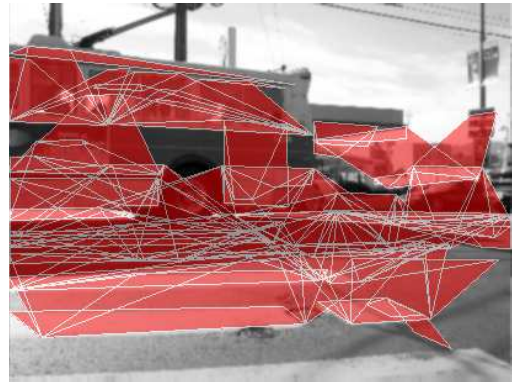
\includegraphics[width=10cm]{figures/CoughlanStriplets.png}
\captionfonts
\caption{Matched top and bottom pairs via the Coughlan Approach \cite{Coughlan2006}}
\label{fig:CoughlanStriplets}
\end{center}
\end{figure}

After matching up pairs of lines into stripelets, many stripelets are found, most of which are not part of the crosswalk (see figure \ref{fig:CoughlanStriplets}).

After extraction, unary and binary cues are used to determine if the stripelets are figure or ground. Their unary cue uses the fact that stripes lower in the image would be wider if they are part of a crosswalk. Coughlan and Shen found a relationship between the vertical width and vertical Y coordinate, as shown in the scatter plot in figure \ref{fig:CoughlanScatter}, a line drawn with a negative slope along a few points with low width and Y value follows the lines that represent stripelets from the crosswalk. They then use a line fitting procedure to try and find an envelope line that fits that model. Once that line is found, they can use it to evaluate other stripelets. They look for longer stripelets that are close to the envelope in order to classify them as potentially a crosswalk stripelet. Additionally, a binary cue is used when the cross ratio test is applied to pairs of stripelets to check that all four lines are approximately parallel. Finally, the cross ratio is also used to verify that adjacent stripelets are within an acceptable distance from each other. 

\begin{figure}[t]
\begin{center}
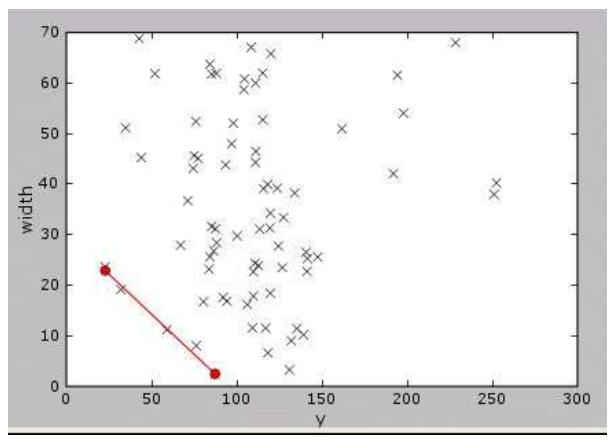
\includegraphics[width=10cm]{figures/CoughlanScatter.png}
\captionfonts
\caption{Scatter plot of vertical Y location and vertical width of stripelets via Coughlan Approach \cite{Coughlan2006}}
\label{fig:CoughlanScatter}
\end{center}
\end{figure}

They ran this algorithm multiple times on each image with different envelope lines, and used the result that had the highest belief value of being correct. Their results are shown in figure \ref{fig:CoughlanResults}. These results were generated in few seconds per image. 

\begin{figure}[t]
\begin{center}
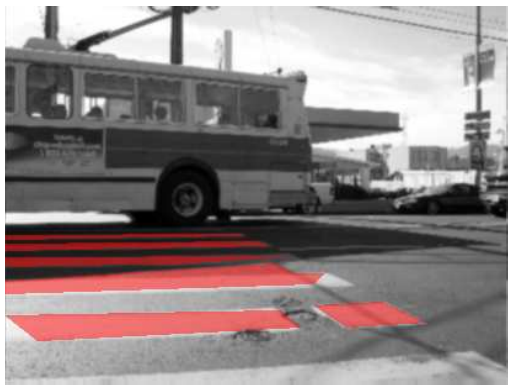
\includegraphics[width=10cm]{figures/CoughlanResult.png}
\captionfonts
\caption{Coughlan Results \cite{Coughlan2006}}
\label{fig:CoughlanResults}
\end{center}
\end{figure}

In their next paper in 2008 \cite{ZebraPhone}, they implemented this algorithm in Symbian C++ on a Nokia  N95 cell phone and obtained a true positive rate of 72\% and a false positive rate of 0.5\% on detected lines being predicted correctly as part of a crosswalk or not over a test set of 30 crosswalk images and 60 non-crosswalk images. Running on their 332 MHz ARM 11 processor running on 320x240 resolution pictures, they were able to obtain a processing speed of three frames per second with optimizations, compared to their processing speed on a PC with unoptimized code, and they believed the code could be further optimized as well. 